\chaptertitle{Chapter 1, des trucs bien}
\label{chap:chap1}
\introformatting

\lettrine{C}{e chapitre} est consacré parler de la chose \suiv.
Est. Donec semper nulla in ipsum. Integer elit. In pharetra lorem vel ante.
Sed sed justo. Curabitur consectetuer arcu. Etiam placerat est eget odio. Nulla
facilisi. Nulla facilisi. Mauris non neque. Suspendisse et diam. Sed vestibulum
malesuada ipsum. Cras id magna. Nunc pharetra velit vitae eros. Vivamus ac
risus. Mauris ac pede laoreet felis pharetra ultricies. Proin et neque. Aliquam
dignissim placerat felis. Mauris porta ante sagittis purus.

Pellentesque quis leo eget ante tempor cursus. Pellentesque sagittis, diam ut
dictum accumsan, magna est viverra erat, vitae imperdiet neque mauris aliquam
nisl. Suspendisse blandit quam quis felis. Praesent turpis nunc, vehicula in,
bibendum vitae, blandit ac, turpis. Duis rhoncus. Vestibulum metus. Morbi
consectetuer felis id tortor. Etiam augue leo, cursus eget, ornare et, ornare
sagittis, tellus. Fusce felis tellus, consectetuer nec, consequat at, ornare
non, arcu. Maecenas condimentum sodales odio. Sed eu orci.

Nullam adipiscing eros sit amet ante. Vestibulum ante. Sed quis ipsum non ligula
dignissim luctus. Integer quis justo id tortor accumsan tempus. Cras vitae
magna. Nunc bibendum lacinia tellus. Quisque porttitor ligula et pede. Nam erat
nibh, fringilla ac, rutrum sit amet, rhoncus in, ipsum. Mauris rhoncus, lacus eu
convallis sagittis, quam magna placerat est, vitae imperdiet mauris arcu ac dui.
In ac urna non justo posuere mattis. Suspendisse egestas bibendum nulla. In erat
nunc, posuere sed, auctor quis, pulvinar quis, mi. Mauris at est. Phasellus
lacinia eros in arcu. Maecenas lobortis, tellus vel gravida tincidunt, elit erat
suscipit arcu, in varius erat risus vel magna. Fusce nec ante quis dolor
vestibulum bibendum. Pellentesque sit amet urna.

Curabitur eget nisi at lectus placerat gravida. Vivamus nulla. Donec luctus. Sed
quis tellus. Quisque lobortis faucibus mi. Aenean vitae risus ut arcu malesuada
ornare. Maecenas nec erat. Sed rhoncus, elit laoreet sagittis luctus, nulla leo
faucibus lectus, vitae accumsan est diam id felis. Nunc dui.
% lorem}}}


\section{Section 1}
\label{sec-section1}

\begin{contenu}

  ici, on va présenter une figure, voir figure~\ref{fig-tool}. Et on va citer
  des articles \cite{torproject, churnMagnienBenamara, cholez2010,
  wikipediaedonkey, edonkey, blecic98, hancock90}. Et, vehicula auctor, iaculis
  id, diam. Morbi viverra neque sit amet risus. Nunc pellentesque aliquam orci.
  Proin neque elit, mollis vel, tristique nec, varius consectetuer, lorem. Nam
  malesuada ornare nunc. Duis turpis turpis, fermentum a, aliquet quis, sodales
  at, dolor. Duis eget velit eget risus fringilla hendrerit. Nulla facilisi.
  Mauris turpis pede, aliquet ac, mattis sed, consequat in, massa. Cum sociis
  natoque penatibus et magnis dis parturient montes, nascetur ridiculus mus.
  Etiam egestas posuere metus. Aliquam erat volutpat. Donec non tortor. Vivamus
  posuere nisi mollis dolor. Quisque porttitor nisi ac elit. Nullam tincidunt
  ligula vitae nulla. 

  \begin{brouillon}
  Vivamus sit amet risus et ipsum viverra malesuada. Duis
  luctus. Curabitur adipiscing metus et felis. Vestibulum tortor. Pellentesque
  purus. Donec pharetra, massa quis malesuada auctor, tortor ipsum lobortis
  ipsum, eget facilisis ante nisi eget lectus. Sed a est. Aliquam nec felis eu
  sem euismod viverra. Suspendisse felis mi, dictum id, convallis ac, mattis
  non, nibh. Donec sagittis quam eu mauris. Phasellus et leo at quam dapibus
  pellentesque. In non lacus. Nullam tristique nunc ut arcu scelerisque aliquam.
  Nullam viverra magna vitae leo. Vestibulum in lacus sit amet lectus tempus
  aliquet. Duis cursus nisl ac orci. Donec non nisl. Mauris lacus sapien, congue
  a, facilisis at, egestas.
  \end{brouillon}


\begin{figure}[!ht]
\centering
%\resizebox{\columnwidth}{!}{
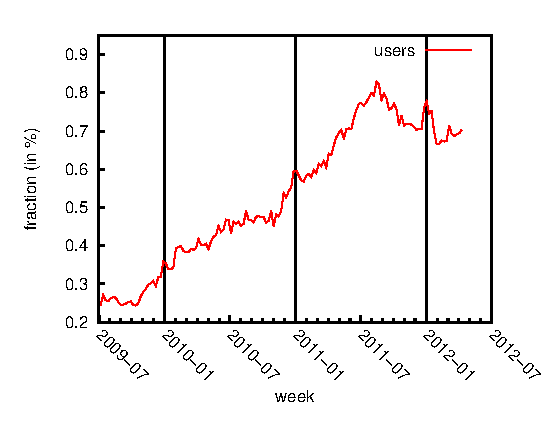
\includegraphics[width=\columnwidth]{anotherthing-week-coul-en.eps}
%}
\caption[Figure bidule]{Ceci est la description de la figure. Les données sont
en annexe~\ref{app:appendice1}} 
\label{fig-tool}
\end{figure}

\end{contenu}

\begin{encadre}
  Dans cette section, on fait ci, puis ça et enfin ça. On est content.
\end{encadre}

\section{Section2}
% lorem{{{
Sapien. Praesent enim mauris, suscipit a, auctor et, lacinia vitae, nunc.
Pellentesque habitant morbi tristique senectus et netus et malesuada fames ac
turpis egestas. Praesent lacus diam, auctor quis, venenatis in, hendrerit at,
est. Vivamus eget eros. Phasellus congue, sapien ac iaculis feugiat, lacus lacus
accumsan lorem, quis volutpat justo turpis ac mauris.

Duis velit magna, scelerisque vitae, varius ut, aliquam vel, justo. Proin ac
augue. Nullam auctor lectus vitae arcu. Vestibulum porta justo placerat purus.
Ut sem nunc, vestibulum nec, sodales vitae, vehicula eget, ipsum. Sed nec
tortor. Aenean malesuada. Nunc convallis, massa eu vestibulum commodo, quam
mauris interdum arcu, at pellentesque diam metus ut nulla. Vestibulum eu dolor
sit amet lacus varius fermentum. Morbi dolor enim, pulvinar eget, lobortis ac,
fringilla ac, turpis. Duis ac erat. Etiam consequat. Integer sed est eu elit
pellentesque dapibus. Duis venenatis magna feugiat nisi. Vestibulum et turpis.
Maecenas a enim. Suspendisse ultricies ornare justo. Fusce sit amet nisi sed
arcu condimentum venenatis. Vivamus dui. Nunc accumsan, quam a fermentum mattis,
magna sapien iaculis pede, at porttitor quam odio at est.

Proin eleifend nisi et nibh. Maecenas a lacus. Mauris porta quam non massa
molestie scelerisque. Nulla sed ante at lorem suscipit rutrum. Nam quis tellus.
Cras elit nisi, ornare a, condimentum vitae, rutrum sit amet, tellus. Maecenas a
dolor. Praesent tempor, felis eget gravida blandit, urna lacus faucibus velit,
in consectetuer sapien erat nec quam. Integer bibendum odio sit amet neque.
Integer imperdiet rhoncus mi. Pellentesque malesuada purus id purus. Quisque
viverra porta lectus. Sed lacus leo, feugiat at, consectetuer eu, luctus quis,
risus. Suspendisse faucibus orci et nunc. Nullam vehicula fermentum risus. Fusce
felis nibh, dignissim vulputate, ultrices quis, lobortis et, arcu. Duis aliquam
libero non diam.

Vestibulum placerat tincidunt tortor. Ut vehicula ligula quis lectus. In eget
velit. Quisque vel risus. Mauris pede. Nullam ornare sapien sit amet nisl. Cras
tortor. Donec tortor lorem, dignissim sit amet, pulvinar eget, mattis eu, metus.
Cras vestibulum erat ultrices neque. Praesent rhoncus, dui blandit pellentesque
congue, mauris mi ullamcorper odio, eget ultricies nunc felis in augue. Nullam
porta nunc. Donec in pede ac mauris mattis eleifend. Cras a libero vel est
lacinia dictum. In hac habitasse platea dictumst. Nullam malesuada molestie
lorem. Nunc non mauris. Nam accumsan tortor gravida elit. Cras porttitor.

Praesent vel enim sed eros luctus imperdiet. Mauris neque ante, placerat at,
mollis vitae, faucibus quis, leo. Ut feugiat. Vivamus urna quam, congue
vulputate, convallis non.
% lorem}}}

\begin{encadre}
  Dans cette section, on fait des trucs.
\end{encadre}

%%%%%%%%%%%%%%%%%%%%%%%%%%%%%%%%%%%%%%%%%

\section{Conclusion}

Dans ce chapitre, nous avons présenté \ldots.
Dans le chapitre~\ref{chap:chap2}, nous ferons ceci, qui est mieux.

\outroformatting
